\chapter{Schemi}
\section{Schemi a Blocchi}
Serve a rappresentare un sistema graficamente dati ingressi e uscite

\begin{example}
	
	dato un segnale $ u(t)=\delta_{-2}(t) $ ottengo un blocco così:
	
	%%%%%%%%%% immagine %%%%%%%
	\begin{center}
			\tikzset{every picture/.style={line width=0.75pt}} %set default line width to 0.75pt        
	
		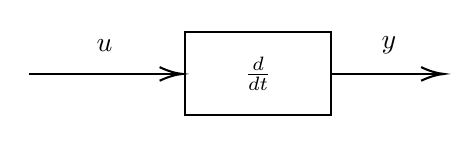
\begin{tikzpicture}[x=0.75pt,y=0.75pt,yscale=-1,xscale=1]
		%uncomment if require: \path (0,59.33332824707031); %set diagram left start at 0, and has height of 59.33332824707031
		
		%Shape: Rectangle [id:dp9183683659728177] 
		\draw   (288,6) -- (358,6) -- (358,46) -- (288,46) -- cycle ;
		%Straight Lines [id:da4783012359570893] 
		\draw    (358,26) -- (410.5,26) ;
		\draw [shift={(412.5,26)}, rotate = 180] [color={rgb, 255:red, 0; green, 0; blue, 0 }  ][line width=0.75]    (10.93,-3.29) .. controls (6.95,-1.4) and (3.31,-0.3) .. (0,0) .. controls (3.31,0.3) and (6.95,1.4) .. (10.93,3.29)   ;
		
		%Straight Lines [id:da8992957067336038] 
		\draw    (212.5,26) -- (284.5,26) ;
		\draw [shift={(286.5,26)}, rotate = 180] [color={rgb, 255:red, 0; green, 0; blue, 0 }  ][line width=0.75]    (10.93,-3.29) .. controls (6.95,-1.4) and (3.31,-0.3) .. (0,0) .. controls (3.31,0.3) and (6.95,1.4) .. (10.93,3.29)   ;
		
		
		% Text Node
		\draw (323,26) node   {$\frac{d}{dt}$};
		% Text Node
		\draw (249,12.32) node   {$u$};
		% Text Node
		\draw (386,12.32) node   {$y$};
		
		\end{tikzpicture}
	\end{center}
	ottengo:  $ y(t)=\delta_{-1}(t) $
\end{example}

\begin{example}
	Sistema massa molla smorzatore
	
	\begin{center}
	
	
	\tikzset{every picture/.style={line width=0.75pt}} %set default line width to 0.75pt        
	
		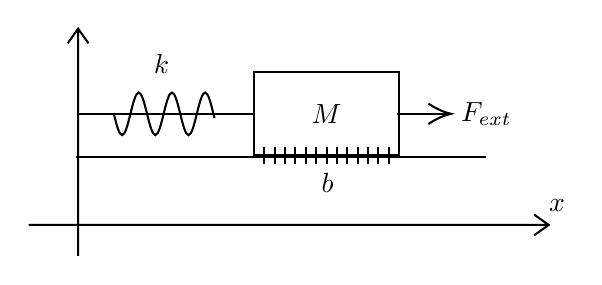
\begin{tikzpicture}[x=0.75pt,y=0.75pt,yscale=-1,xscale=1]
		%uncomment if require: \path (0,509); %set diagram left start at 0, and has height of 509
		
		%Shape: Axis 2D [id:dp2949613832069744] 
		\draw  (208,184.53) -- (458.5,184.53)(231.8,90) -- (231.8,199.5) (451.5,179.53) -- (458.5,184.53) -- (451.5,189.53) (226.8,97) -- (231.8,90) -- (236.8,97)  ;
		%Shape: Rectangle [id:dp8682403506536873] 
		\draw   (316.5,111) -- (386.5,111) -- (386.5,151) -- (316.5,151) -- cycle ;
		%Straight Lines [id:da4773229437516673] 
		\draw    (232,131) -- (316,131) ;
		
		
		%Shape: Wave [id:dp5588027634095529] 
		\draw   (249,131) .. controls (250.3,136.25) and (251.55,141.25) .. (253,141.25) .. controls (254.45,141.25) and (255.7,136.25) .. (257,131) .. controls (258.3,125.75) and (259.55,120.75) .. (261,120.75) .. controls (262.45,120.75) and (263.7,125.75) .. (265,131) .. controls (266.3,136.25) and (267.55,141.25) .. (269,141.25) .. controls (270.45,141.25) and (271.7,136.25) .. (273,131) .. controls (274.3,125.75) and (275.55,120.75) .. (277,120.75) .. controls (278.45,120.75) and (279.7,125.75) .. (281,131) .. controls (282.3,136.25) and (283.55,141.25) .. (285,141.25) .. controls (286.45,141.25) and (287.7,136.25) .. (289,131) .. controls (290.3,125.75) and (291.55,120.75) .. (293,120.75) .. controls (294.45,120.75) and (295.7,125.75) .. (297,131) .. controls (297.17,131.67) and (297.33,132.34) .. (297.5,133) ;
		%Straight Lines [id:da6778535466302025] 
		\draw    (231,152) -- (428.5,152) ;
		
		%Straight Lines [id:da06443124093800989] 
		\draw    (385.5,131) -- (409.5,131) ;
		\draw [shift={(411.5,131)}, rotate = 180] [color={rgb, 255:red, 0; green, 0; blue, 0 }  ][line width=0.75]    (10.93,-4.9) .. controls (6.95,-2.3) and (3.31,-0.67) .. (0,0) .. controls (3.31,0.67) and (6.95,2.3) .. (10.93,4.9)   ;
		
		%Straight Lines [id:da47502722033668277] 
		\draw    (316.5,151) -- (386.5,151) (321.5,147) -- (321.5,155)(326.5,147) -- (326.5,155)(331.5,147) -- (331.5,155)(336.5,147) -- (336.5,155)(341.5,147) -- (341.5,155)(346.5,147) -- (346.5,155)(351.5,147) -- (351.5,155)(356.5,147) -- (356.5,155)(361.5,147) -- (361.5,155)(366.5,147) -- (366.5,155)(371.5,147) -- (371.5,155)(376.5,147) -- (376.5,155)(381.5,147) -- (381.5,155) ;		
		
		% Text Node
		\draw (351.5,131) node   {$M$};
		% Text Node
		\draw (272,107) node   {$k$};
		% Text Node
		\draw (352,164.5) node   {$b$};
		% Text Node
		\draw (428.5,131) node   {$F_{ext}$};
		% Text Node
		\draw (462.5,175) node   {$x$};
	\end{tikzpicture}
	\end{center}

	con $ k $ costante della molla, $ f_{ext} $ forza applicata, $ M $ massa e $ b $ attrito.
	
	Scriviamo l'equazione del sistema in riferimento alla posizione $ x $ ricordandoci che la velocità è la prima derivata dello spazio mentre l'accellerazione ne è la seconda:
	\[
		\sum F = M \cdot a \Rightarrow F_{ext}-kx-bx'= Mx'' \Rightarrow F_{ext}=kx+bx'+ Mx''
	\]
	\[
		\LA \rightarrow F_{ext}=kX(s)+sbX(s)+ s^2MX(s) 
		= X(s) (k+sb+s^2M) \Rightarrow X(s)=F_{ext} \frac{1}{k+sb+s^2M}
	\]
	
	Trasformiamo nello schema a blocchi:
	
	\begin{center}
		\tikzset{every picture/.style={line width=0.75pt}} %set default line width to 0.75pt        
		
		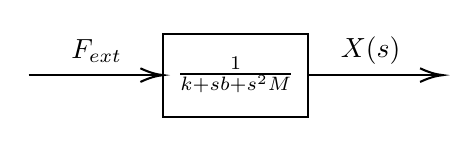
\begin{tikzpicture}[x=0.75pt,y=0.75pt,yscale=-1,xscale=1]
		%uncomment if require: \path (0,300); %set diagram left start at 0, and has height of 300
		
		%Shape: Rectangle [id:dp6464909345742553] 
		\draw   (285,103) -- (355,103) -- (355,143) -- (285,143) -- cycle ;
		%Straight Lines [id:da3909182970545064] 
		\draw    (220.25,123) -- (283,123) ;
		\draw [shift={(285,123)}, rotate = 180] [color={rgb, 255:red, 0; green, 0; blue, 0 }  ][line width=0.75]    (10.93,-3.29) .. controls (6.95,-1.4) and (3.31,-0.3) .. (0,0) .. controls (3.31,0.3) and (6.95,1.4) .. (10.93,3.29)   ;
		
		%Straight Lines [id:da20464322978360183] 
		\draw    (355,123) -- (417.75,123) ;
		\draw [shift={(419.75,123)}, rotate = 180] [color={rgb, 255:red, 0; green, 0; blue, 0 }  ][line width=0.75]    (10.93,-3.29) .. controls (6.95,-1.4) and (3.31,-0.3) .. (0,0) .. controls (3.31,0.3) and (6.95,1.4) .. (10.93,3.29)   ;
		
		
		% Text Node
		\draw (320,123) node   {$\frac{1}{k+sb+s^{2} M}$};
		% Text Node
		\draw (253,111.25) node   {$F_{ext}$};
		% Text Node
		\draw (385,111.25) node   {$X( s)$};
		\end{tikzpicture}
	\end{center}
\end{example}

\subsection{Diagramma ad anello chiuso}

Se l'ingresso non dipende dall'uscita si dice ad \emph{Anello Aperto}, altrimenti ad \emph{Anello Chiuso} (o retroazionato). Quest'ultimo è quello più usato.

\begin{center}
	\tikzset{every picture/.style={line width=0.75pt}} %set default line width to 0.75pt        
	
	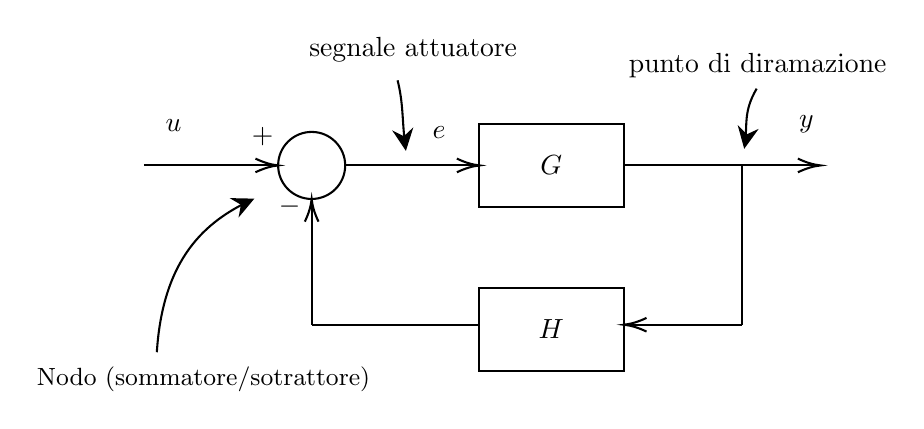
\begin{tikzpicture}[x=0.75pt,y=0.75pt,yscale=-1,xscale=1]
	%uncomment if require: \path (0,292); %set diagram left start at 0, and has height of 292
	
	%Shape: Rectangle [id:dp3155084585495189] 
	\draw   (324.5,123) -- (394.5,123) -- (394.5,163) -- (324.5,163) -- cycle ;
	%Straight Lines [id:da11063592261012656] 
	\draw    (260.25,143) -- (323,143) ;
	\draw [shift={(325,143)}, rotate = 180] [color={rgb, 255:red, 0; green, 0; blue, 0 }  ][line width=0.75]    (10.93,-3.29) .. controls (6.95,-1.4) and (3.31,-0.3) .. (0,0) .. controls (3.31,0.3) and (6.95,1.4) .. (10.93,3.29)   ;
	
	%Straight Lines [id:da8163995279030745] 
	\draw    (395,143) -- (487.3,143) ;
	\draw [shift={(489.3,143)}, rotate = 180] [color={rgb, 255:red, 0; green, 0; blue, 0 }  ][line width=0.75]    (10.93,-3.29) .. controls (6.95,-1.4) and (3.31,-0.3) .. (0,0) .. controls (3.31,0.3) and (6.95,1.4) .. (10.93,3.29)   ;
	
	%Flowchart: Connector [id:dp7546342860954656] 
	\draw   (227.95,143) .. controls (227.95,134.08) and (235.18,126.85) .. (244.1,126.85) .. controls (253.02,126.85) and (260.25,134.08) .. (260.25,143) .. controls (260.25,151.92) and (253.02,159.15) .. (244.1,159.15) .. controls (235.18,159.15) and (227.95,151.92) .. (227.95,143) -- cycle ;
	%Straight Lines [id:da6036888305055024] 
	\draw    (163.2,143) -- (225.95,143) ;
	\draw [shift={(227.95,143)}, rotate = 180] [color={rgb, 255:red, 0; green, 0; blue, 0 }  ][line width=0.75]    (10.93,-3.29) .. controls (6.95,-1.4) and (3.31,-0.3) .. (0,0) .. controls (3.31,0.3) and (6.95,1.4) .. (10.93,3.29)   ;
	
	%Straight Lines [id:da10222491957386626] 
	\draw    (244.1,219.75) -- (244.1,161.15) ;
	\draw [shift={(244.1,159.15)}, rotate = 450] [color={rgb, 255:red, 0; green, 0; blue, 0 }  ][line width=0.75]    (10.93,-3.29) .. controls (6.95,-1.4) and (3.31,-0.3) .. (0,0) .. controls (3.31,0.3) and (6.95,1.4) .. (10.93,3.29)   ;
	
	%Shape: Rectangle [id:dp3211173615588092] 
	\draw   (324.5,202) -- (394.5,202) -- (394.5,242) -- (324.5,242) -- cycle ;
	%Straight Lines [id:da42233637174500327] 
	\draw    (244.1,219.75) -- (324.3,219.75) ;
	
	
	%Straight Lines [id:da9688852904709178] 
	\draw    (396.5,219.75) -- (451.3,219.75) ;
	
	\draw [shift={(394.5,219.75)}, rotate = 0] [color={rgb, 255:red, 0; green, 0; blue, 0 }  ][line width=0.75]    (10.93,-3.29) .. controls (6.95,-1.4) and (3.31,-0.3) .. (0,0) .. controls (3.31,0.3) and (6.95,1.4) .. (10.93,3.29)   ;
	%Straight Lines [id:da49473026564794287] 
	\draw    (451.3,143) -- (451.3,219.75) ;
	
	
	%Curve Lines [id:da6898335310358139] 
	\draw    (285.5,102) .. controls (288.37,113.46) and (287.58,121.27) .. (289.25,134.15) ;
	\draw [shift={(289.5,136)}, rotate = 261.87] [fill={rgb, 255:red, 0; green, 0; blue, 0 }  ][line width=0.75]  [draw opacity=0] (10.72,-5.15) -- (0,0) -- (10.72,5.15) -- (7.12,0) -- cycle    ;
	
	%Curve Lines [id:da7097329155318699] 
	\draw    (458.5,106) .. controls (451.92,117.28) and (454.18,123.26) .. (452.81,133.07) ;
	\draw [shift={(452.5,135)}, rotate = 280.3] [fill={rgb, 255:red, 0; green, 0; blue, 0 }  ][line width=0.75]  [draw opacity=0] (10.72,-5.15) -- (0,0) -- (10.72,5.15) -- (7.12,0) -- cycle    ;
	
	%Curve Lines [id:da6339380725476107] 
	\draw    (169.5,233) .. controls (172.43,187.17) and (193.41,169.87) .. (214.85,159.76) ;
	\draw [shift={(216.5,159)}, rotate = 515.56] [fill={rgb, 255:red, 0; green, 0; blue, 0 }  ][line width=0.75]  [draw opacity=0] (10.72,-5.15) -- (0,0) -- (10.72,5.15) -- (7.12,0) -- cycle    ;
	
	
	% Text Node
	\draw (359.5,143) node   {$G$};
	% Text Node
	\draw (359.5,222) node   {$H$};
	% Text Node
	\draw (177.5,124) node   {$u$};
	% Text Node
	\draw (482.5,123) node   {$y$};
	% Text Node
	\draw (220.5,129) node   {$+$};
	% Text Node
	\draw (233.5,163) node   {$-$};
	% Text Node
	\draw (192,246) node  [align=left] {{\small Nodo (sommatore/sotrattore)}};
	% Text Node
	\draw (459,95) node  [align=left] {punto di diramazione};
	% Text Node
	\draw (293,87) node  [align=left] {segnale attuatore};
	% Text Node
	\draw (305.5,127) node   {$e$};
	
	\end{tikzpicture}
\end{center}	
	con $ u $ segnale di riferimento, $ G $ controllore e $ H $ elemento di retroazione. Il segnale attuatore è: $ e(t)=u(t)-Hy(t) $
	
\subsection{Segnali di disturbo}

Possono esserci dei segnali di disturbo in entrata. In questo caso prima si trova $ y $ esclusivamente in funzione di $ u $ poi esclusivamente in funzione di $ d $. %TODO: controllare se vera

\begin{center}
	
	
	\tikzset{every picture/.style={line width=0.75pt}} %set default line width to 0.75pt        
	
	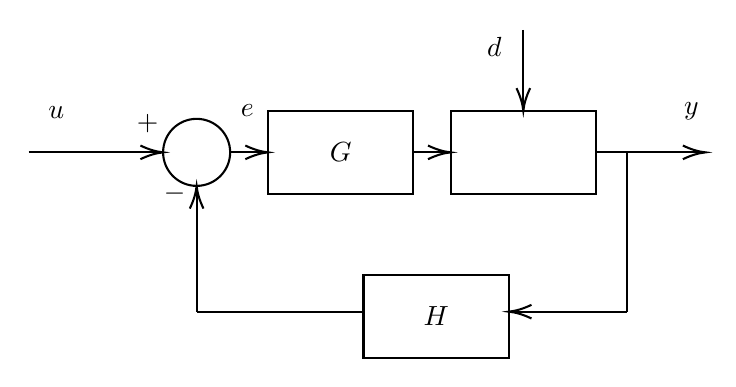
\begin{tikzpicture}[x=0.75pt,y=0.75pt,yscale=-1,xscale=1]
	%uncomment if require: \path (0,300); %set diagram left start at 0, and has height of 300
	
	%Shape: Rectangle [id:dp8002427712904623] 
	\draw   (280.5,107) -- (350.5,107) -- (350.5,147) -- (280.5,147) -- cycle ;
	%Straight Lines [id:da652142321436137] 
	\draw    (262.25,127) -- (278.5,127) ;
	\draw [shift={(280.5,127)}, rotate = 180] [color={rgb, 255:red, 0; green, 0; blue, 0 }  ][line width=0.75]    (10.93,-3.29) .. controls (6.95,-1.4) and (3.31,-0.3) .. (0,0) .. controls (3.31,0.3) and (6.95,1.4) .. (10.93,3.29)   ;
	
	%Straight Lines [id:da980428882327369] 
	\draw    (438.5,127) -- (489.3,127) ;
	\draw [shift={(491.3,127)}, rotate = 180] [color={rgb, 255:red, 0; green, 0; blue, 0 }  ][line width=0.75]    (10.93,-3.29) .. controls (6.95,-1.4) and (3.31,-0.3) .. (0,0) .. controls (3.31,0.3) and (6.95,1.4) .. (10.93,3.29)   ;
	
	%Flowchart: Connector [id:dp7103967563362967] 
	\draw   (229.95,127) .. controls (229.95,118.08) and (237.18,110.85) .. (246.1,110.85) .. controls (255.02,110.85) and (262.25,118.08) .. (262.25,127) .. controls (262.25,135.92) and (255.02,143.15) .. (246.1,143.15) .. controls (237.18,143.15) and (229.95,135.92) .. (229.95,127) -- cycle ;
	%Straight Lines [id:da39229442705370654] 
	\draw    (165.2,127) -- (227.95,127) ;
	\draw [shift={(229.95,127)}, rotate = 180] [color={rgb, 255:red, 0; green, 0; blue, 0 }  ][line width=0.75]    (10.93,-3.29) .. controls (6.95,-1.4) and (3.31,-0.3) .. (0,0) .. controls (3.31,0.3) and (6.95,1.4) .. (10.93,3.29)   ;
	
	%Straight Lines [id:da7835139153281818] 
	\draw    (246.1,203.75) -- (246.1,145.15) ;
	\draw [shift={(246.1,143.15)}, rotate = 450] [color={rgb, 255:red, 0; green, 0; blue, 0 }  ][line width=0.75]    (10.93,-3.29) .. controls (6.95,-1.4) and (3.31,-0.3) .. (0,0) .. controls (3.31,0.3) and (6.95,1.4) .. (10.93,3.29)   ;
	
	%Shape: Rectangle [id:dp14775199124860605] 
	\draw   (326.5,186) -- (396.5,186) -- (396.5,226) -- (326.5,226) -- cycle ;
	%Straight Lines [id:da3771415417056869] 
	\draw    (246.1,203.75) -- (326.3,203.75) ;
	
	
	%Straight Lines [id:da585328914471497] 
	\draw    (398.5,203.75) -- (453.3,203.75) ;
	
	\draw [shift={(396.5,203.75)}, rotate = 0] [color={rgb, 255:red, 0; green, 0; blue, 0 }  ][line width=0.75]    (10.93,-3.29) .. controls (6.95,-1.4) and (3.31,-0.3) .. (0,0) .. controls (3.31,0.3) and (6.95,1.4) .. (10.93,3.29)   ;
	%Straight Lines [id:da29894491742670404] 
	\draw    (453.3,127) -- (453.3,203.75) ;
	
	
	%Shape: Rectangle [id:dp719324064196792] 
	\draw   (368.5,107) -- (438.5,107) -- (438.5,147) -- (368.5,147) -- cycle ;
	%Straight Lines [id:da3308344355409414] 
	\draw    (350.5,127) -- (366.5,127) ;
	\draw [shift={(368.5,127)}, rotate = 180] [color={rgb, 255:red, 0; green, 0; blue, 0 }  ][line width=0.75]    (10.93,-3.29) .. controls (6.95,-1.4) and (3.31,-0.3) .. (0,0) .. controls (3.31,0.3) and (6.95,1.4) .. (10.93,3.29)   ;
	
	%Straight Lines [id:da19666294752409486] 
	\draw    (403.5,68) -- (403.5,105) ;
	\draw [shift={(403.5,107)}, rotate = 270] [color={rgb, 255:red, 0; green, 0; blue, 0 }  ][line width=0.75]    (10.93,-3.29) .. controls (6.95,-1.4) and (3.31,-0.3) .. (0,0) .. controls (3.31,0.3) and (6.95,1.4) .. (10.93,3.29)   ;
	
	
	% Text Node
	\draw (315.5,127) node   {$G$};
	% Text Node
	\draw (361.5,206) node   {$H$};
	% Text Node
	\draw (270.5,107) node   {$e$};
	% Text Node
	\draw (484.5,107) node   {$y$};
	% Text Node
	\draw (222.5,113) node   {$+$};
	% Text Node
	\draw (235.5,147) node   {$-$};
	% Text Node
	\draw (178.5,108) node   {$u$};
	% Text Node
	\draw (389.5,76) node   {$d$};
	
	
	\end{tikzpicture}
\end{center}

\section{Risoluzione di sistemi a Blocchi}
In caso di sistemi complessi è più facile ottenere il sistema risultante tramite trasformazioni di blocchi più piccoli.

\subsection{Blocchi in serie/cascata}
\begin{center}
	
	
	\tikzset{every picture/.style={line width=0.75pt}} %set default line width to 0.75pt        
	
	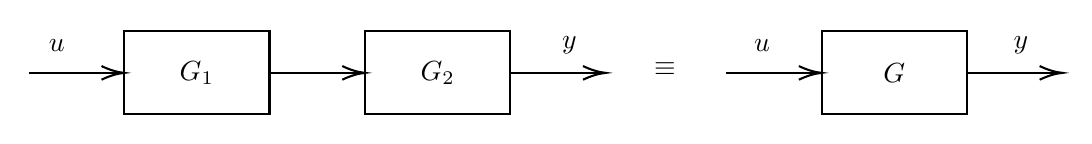
\begin{tikzpicture}[x=0.75pt,y=0.75pt,yscale=-1,xscale=1]
	%uncomment if require: \path (0,106); %set diagram left start at 0, and has height of 106
	
	%Shape: Rectangle [id:dp06254604466462199] 
	\draw   (112.5,24.5) -- (182.5,24.5) -- (182.5,64.5) -- (112.5,64.5) -- cycle ;
	%Shape: Rectangle [id:dp7300837861868514] 
	\draw   (228.5,24.5) -- (298.5,24.5) -- (298.5,64.5) -- (228.5,64.5) -- cycle ;
	%Straight Lines [id:da6782971117734584] 
	\draw    (182.5,44.5) -- (226.5,44.5) ;
	\draw [shift={(228.5,44.5)}, rotate = 180] [color={rgb, 255:red, 0; green, 0; blue, 0 }  ][line width=0.75]    (10.93,-3.29) .. controls (6.95,-1.4) and (3.31,-0.3) .. (0,0) .. controls (3.31,0.3) and (6.95,1.4) .. (10.93,3.29)   ;
	
	%Straight Lines [id:da6363591162519446] 
	\draw    (298.5,44.5) -- (342.5,44.5) ;
	\draw [shift={(344.5,44.5)}, rotate = 180] [color={rgb, 255:red, 0; green, 0; blue, 0 }  ][line width=0.75]    (10.93,-3.29) .. controls (6.95,-1.4) and (3.31,-0.3) .. (0,0) .. controls (3.31,0.3) and (6.95,1.4) .. (10.93,3.29)   ;
	
	%Straight Lines [id:da5764037506135491] 
	\draw    (66.5,44.5) -- (110.5,44.5) ;
	\draw [shift={(112.5,44.5)}, rotate = 180] [color={rgb, 255:red, 0; green, 0; blue, 0 }  ][line width=0.75]    (10.93,-3.29) .. controls (6.95,-1.4) and (3.31,-0.3) .. (0,0) .. controls (3.31,0.3) and (6.95,1.4) .. (10.93,3.29)   ;
	
	%Shape: Rectangle [id:dp8193844196572095] 
	\draw   (448.5,24.5) -- (518.5,24.5) -- (518.5,64.5) -- (448.5,64.5) -- cycle ;
	%Straight Lines [id:da28598519675474865] 
	\draw    (518.5,44.5) -- (562.5,44.5) ;
	\draw [shift={(564.5,44.5)}, rotate = 180] [color={rgb, 255:red, 0; green, 0; blue, 0 }  ][line width=0.75]    (10.93,-3.29) .. controls (6.95,-1.4) and (3.31,-0.3) .. (0,0) .. controls (3.31,0.3) and (6.95,1.4) .. (10.93,3.29)   ;
	
	%Straight Lines [id:da26764641536519096] 
	\draw    (402.5,44.5) -- (446.5,44.5) ;
	\draw [shift={(448.5,44.5)}, rotate = 180] [color={rgb, 255:red, 0; green, 0; blue, 0 }  ][line width=0.75]    (10.93,-3.29) .. controls (6.95,-1.4) and (3.31,-0.3) .. (0,0) .. controls (3.31,0.3) and (6.95,1.4) .. (10.93,3.29)   ;
	
	
	% Text Node
	\draw (147.5,44.5) node   {$G_{1}$};
	% Text Node
	\draw (263.5,44.5) node   {$G_{2}$};
	% Text Node
	\draw (483.5,44.5) node   {$G$};
	% Text Node
	\draw (373,42.67) node   {$\equiv $};
	% Text Node
	\draw (80,31.33) node   {$u$};
	% Text Node
	\draw (327,31.33) node   {$y$};
	% Text Node
	\draw (419.84,31.33) node   {$u$};
	% Text Node
	\draw (544.52,31.33) node   {$y$};
	
	
	\end{tikzpicture}
\end{center}

\[
	G=G_1 \cdot G_2
\]

\subsection{Blocchi in parallelo}
\begin{center}
	
	
	\tikzset{every picture/.style={line width=0.75pt}} %set default line width to 0.75pt        
	
	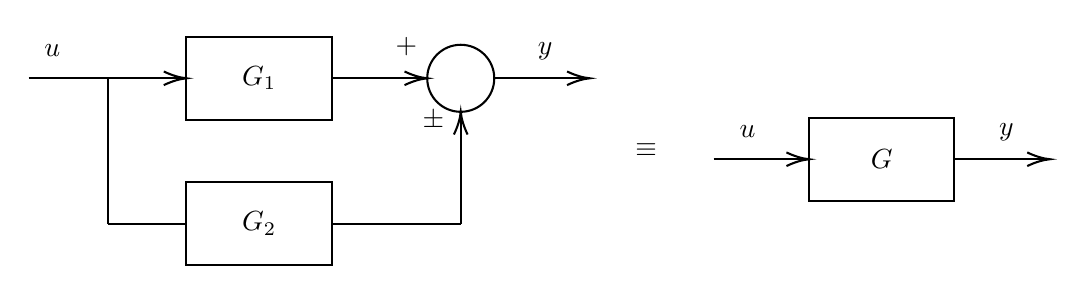
\begin{tikzpicture}[x=0.75pt,y=0.75pt,yscale=-1,xscale=1]
	%uncomment if require: \path (0,156.66665649414062); %set diagram left start at 0, and has height of 156.66665649414062
	
	%Shape: Rectangle [id:dp2537797370216679] 
	\draw   (153.5,26.5) -- (223.5,26.5) -- (223.5,66.5) -- (153.5,66.5) -- cycle ;
	%Shape: Rectangle [id:dp008849470703853113] 
	\draw   (153.5,96.5) -- (223.5,96.5) -- (223.5,136.5) -- (153.5,136.5) -- cycle ;
	%Straight Lines [id:da920241196233377] 
	\draw    (223.5,46.5) -- (267.5,46.5) ;
	\draw [shift={(269.5,46.5)}, rotate = 180] [color={rgb, 255:red, 0; green, 0; blue, 0 }  ][line width=0.75]    (10.93,-3.29) .. controls (6.95,-1.4) and (3.31,-0.3) .. (0,0) .. controls (3.31,0.3) and (6.95,1.4) .. (10.93,3.29)   ;
	
	%Straight Lines [id:da3956988512580457] 
	\draw    (301.8,46.5) -- (345.8,46.5) ;
	\draw [shift={(347.8,46.5)}, rotate = 180] [color={rgb, 255:red, 0; green, 0; blue, 0 }  ][line width=0.75]    (10.93,-3.29) .. controls (6.95,-1.4) and (3.31,-0.3) .. (0,0) .. controls (3.31,0.3) and (6.95,1.4) .. (10.93,3.29)   ;
	
	%Straight Lines [id:da45330941436301075] 
	\draw    (77.5,46.5) -- (151.5,46.5) ;
	\draw [shift={(153.5,46.5)}, rotate = 180] [color={rgb, 255:red, 0; green, 0; blue, 0 }  ][line width=0.75]    (10.93,-3.29) .. controls (6.95,-1.4) and (3.31,-0.3) .. (0,0) .. controls (3.31,0.3) and (6.95,1.4) .. (10.93,3.29)   ;
	
	%Shape: Rectangle [id:dp7875612791922739] 
	\draw   (453.5,65.5) -- (523.5,65.5) -- (523.5,105.5) -- (453.5,105.5) -- cycle ;
	%Straight Lines [id:da4998467873740766] 
	\draw    (523.5,85.5) -- (567.5,85.5) ;
	\draw [shift={(569.5,85.5)}, rotate = 180] [color={rgb, 255:red, 0; green, 0; blue, 0 }  ][line width=0.75]    (10.93,-3.29) .. controls (6.95,-1.4) and (3.31,-0.3) .. (0,0) .. controls (3.31,0.3) and (6.95,1.4) .. (10.93,3.29)   ;
	
	%Straight Lines [id:da869726945090177] 
	\draw    (407.5,85.5) -- (451.5,85.5) ;
	\draw [shift={(453.5,85.5)}, rotate = 180] [color={rgb, 255:red, 0; green, 0; blue, 0 }  ][line width=0.75]    (10.93,-3.29) .. controls (6.95,-1.4) and (3.31,-0.3) .. (0,0) .. controls (3.31,0.3) and (6.95,1.4) .. (10.93,3.29)   ;
	
	%Flowchart: Connector [id:dp37886477247374284] 
	\draw   (269.5,46.5) .. controls (269.5,37.58) and (276.73,30.35) .. (285.65,30.35) .. controls (294.57,30.35) and (301.8,37.58) .. (301.8,46.5) .. controls (301.8,55.42) and (294.57,62.65) .. (285.65,62.65) .. controls (276.73,62.65) and (269.5,55.42) .. (269.5,46.5) -- cycle ;
	%Straight Lines [id:da4643477020568181] 
	\draw    (285.65,116.5) -- (285.65,64.65) ;
	\draw [shift={(285.65,62.65)}, rotate = 450] [color={rgb, 255:red, 0; green, 0; blue, 0 }  ][line width=0.75]    (10.93,-3.29) .. controls (6.95,-1.4) and (3.31,-0.3) .. (0,0) .. controls (3.31,0.3) and (6.95,1.4) .. (10.93,3.29)   ;
	
	%Straight Lines [id:da15310891193572584] 
	\draw    (223.5,116.5) -- (285.65,116.5) ;
	
	
	%Straight Lines [id:da24531771565102178] 
	\draw    (115.5,116.5) -- (153.5,116.5) ;
	
	
	%Straight Lines [id:da6554585448291919] 
	\draw    (115.5,116.5) -- (115.5,46.5) ;
	
	
	
	% Text Node
	\draw (188.5,46.5) node   {$G_{1}$};
	% Text Node
	\draw (188.5,116.5) node   {$G_{2}$};
	% Text Node
	\draw (488.5,85.5) node   {$G$};
	% Text Node
	\draw (259.5,31) node   {$+$};
	% Text Node
	\draw (272.5,67) node   {$\pm $};
	% Text Node
	\draw (375,81) node   {$\equiv $};
	% Text Node
	\draw (423.84,72.33) node   {$u$};
	% Text Node
	\draw (548.52,72.33) node   {$y$};
	% Text Node
	\draw (88.91,33.33) node   {$u$};
	% Text Node
	\draw (326.28,33.33) node   {$y$};
	
	
	\end{tikzpicture}
\end{center}

\[
G=G_1 \pm G_2
\]


\subsection{Sistema retroazionato}
\begin{center}


\tikzset{every picture/.style={line width=0.75pt}} %set default line width to 0.75pt        

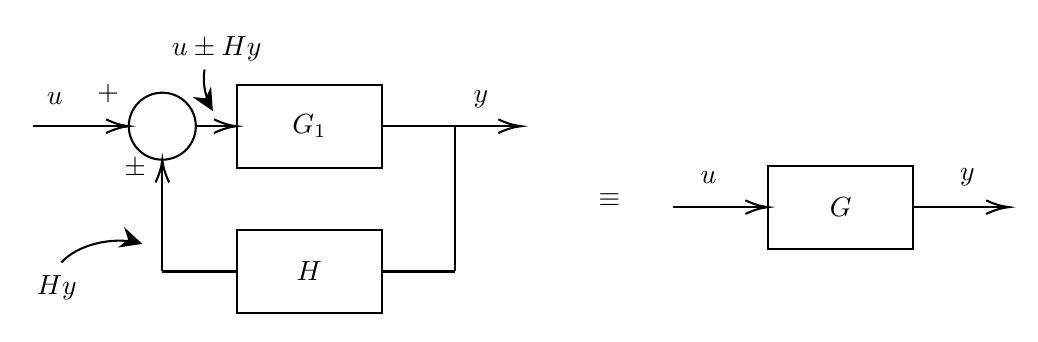
\begin{tikzpicture}[x=0.75pt,y=0.75pt,yscale=-1,xscale=1]
%uncomment if require: \path (0,171.66665649414062); %set diagram left start at 0, and has height of 171.66665649414062

%Shape: Rectangle [id:dp3240175156841656] 
\draw   (181.5,33.5) -- (251.5,33.5) -- (251.5,73.5) -- (181.5,73.5) -- cycle ;
%Shape: Rectangle [id:dp6608672243845539] 
\draw   (181.5,103.5) -- (251.5,103.5) -- (251.5,143.5) -- (181.5,143.5) -- cycle ;
%Straight Lines [id:da4887381227487937] 
\draw    (83.5,53.5) -- (127.5,53.5) ;
\draw [shift={(129.5,53.5)}, rotate = 180] [color={rgb, 255:red, 0; green, 0; blue, 0 }  ][line width=0.75]    (10.93,-3.29) .. controls (6.95,-1.4) and (3.31,-0.3) .. (0,0) .. controls (3.31,0.3) and (6.95,1.4) .. (10.93,3.29)   ;

%Straight Lines [id:da3576050474057568] 
\draw    (251.8,53.5) -- (316.5,53.5) ;
\draw [shift={(318.5,53.5)}, rotate = 180] [color={rgb, 255:red, 0; green, 0; blue, 0 }  ][line width=0.75]    (10.93,-3.29) .. controls (6.95,-1.4) and (3.31,-0.3) .. (0,0) .. controls (3.31,0.3) and (6.95,1.4) .. (10.93,3.29)   ;

%Straight Lines [id:da5570207424626268] 
\draw    (161.8,53.5) -- (179.5,53.5) ;
\draw [shift={(181.5,53.5)}, rotate = 180] [color={rgb, 255:red, 0; green, 0; blue, 0 }  ][line width=0.75]    (10.93,-3.29) .. controls (6.95,-1.4) and (3.31,-0.3) .. (0,0) .. controls (3.31,0.3) and (6.95,1.4) .. (10.93,3.29)   ;

%Shape: Rectangle [id:dp9512547434168017] 
\draw   (437.5,72.5) -- (507.5,72.5) -- (507.5,112.5) -- (437.5,112.5) -- cycle ;
%Straight Lines [id:da9547629996502616] 
\draw    (507.5,92.5) -- (551.5,92.5) ;
\draw [shift={(553.5,92.5)}, rotate = 180] [color={rgb, 255:red, 0; green, 0; blue, 0 }  ][line width=0.75]    (10.93,-3.29) .. controls (6.95,-1.4) and (3.31,-0.3) .. (0,0) .. controls (3.31,0.3) and (6.95,1.4) .. (10.93,3.29)   ;

%Straight Lines [id:da4329180015438556] 
\draw    (391.5,92.5) -- (435.5,92.5) ;
\draw [shift={(437.5,92.5)}, rotate = 180] [color={rgb, 255:red, 0; green, 0; blue, 0 }  ][line width=0.75]    (10.93,-3.29) .. controls (6.95,-1.4) and (3.31,-0.3) .. (0,0) .. controls (3.31,0.3) and (6.95,1.4) .. (10.93,3.29)   ;

%Flowchart: Connector [id:dp15383669633858665] 
\draw   (129.5,53.5) .. controls (129.5,44.58) and (136.73,37.35) .. (145.65,37.35) .. controls (154.57,37.35) and (161.8,44.58) .. (161.8,53.5) .. controls (161.8,62.42) and (154.57,69.65) .. (145.65,69.65) .. controls (136.73,69.65) and (129.5,62.42) .. (129.5,53.5) -- cycle ;
%Straight Lines [id:da4738477696597776] 
\draw    (145.65,123.5) -- (145.65,71.65) ;
\draw [shift={(145.65,69.65)}, rotate = 450] [color={rgb, 255:red, 0; green, 0; blue, 0 }  ][line width=0.75]    (10.93,-3.29) .. controls (6.95,-1.4) and (3.31,-0.3) .. (0,0) .. controls (3.31,0.3) and (6.95,1.4) .. (10.93,3.29)   ;

%Straight Lines [id:da24258510778213926] 
\draw    (251.5,123.5) -- (286.5,123.5) ;


%Straight Lines [id:da3046422054343556] 
\draw    (145.65,123.5) -- (181.5,123.5) ;


%Straight Lines [id:da9939745193683625] 
\draw    (286.5,123.5) -- (286.5,53.5) ;


%Curve Lines [id:da24015808420977258] 
\draw    (97,119.2) .. controls (104.64,110.6) and (121.4,106.57) .. (134.22,109.7) ;
\draw [shift={(136,110.2)}, rotate = 197.1] [fill={rgb, 255:red, 0; green, 0; blue, 0 }  ][line width=0.75]  [draw opacity=0] (10.72,-5.15) -- (0,0) -- (10.72,5.15) -- (7.12,0) -- cycle    ;

%Curve Lines [id:da6376172389939263] 
\draw    (166,26.2) .. controls (165.08,31.72) and (165.85,38.08) .. (169.1,44.52) ;
\draw [shift={(170,46.2)}, rotate = 240.26] [fill={rgb, 255:red, 0; green, 0; blue, 0 }  ][line width=0.75]  [draw opacity=0] (10.72,-5.15) -- (0,0) -- (10.72,5.15) -- (7.12,0) -- cycle    ;


% Text Node
\draw (216.5,53.5) node   {$G_{1}$};
% Text Node
\draw (216.5,123.5) node   {$H$};
% Text Node
\draw (472.5,92.5) node   {$G$};
% Text Node
\draw (119.5,38) node   {$+$};
% Text Node
\draw (132.5,74) node   {$\pm $};
% Text Node
\draw (361,89) node   {$\equiv $};
% Text Node
\draw (408.84,78.33) node   {$u$};
% Text Node
\draw (533.52,78.33) node   {$y$};
% Text Node
\draw (93.82,40.33) node   {$u$};
% Text Node
\draw (299.18,40.33) node   {$y$};
% Text Node
\draw (94.82,131.33) node   {$Hy$};
% Text Node
\draw (171.82,16.33) node   {$u\pm Hy$};


\end{tikzpicture}
\end{center}
\[
	y= G_1(u \pm Hy) 
	\Rightarrow y = G_1 u \pm G_1 Hy
	\Rightarrow y \mp G_1 Hy= G_1 u 
	\Rightarrow y(1\mp G_1 H)= G_1 u
	\Rightarrow y= \frac{G_1 u}{1\mp G_1 H}	
\]
\[
	G = \frac{G_1 }{1\mp G_1 H}
\]
%TODO controllare segni disegno e formula

\subsection{Retroazione unitaria}
\begin{center}
	
	
	\tikzset{every picture/.style={line width=0.75pt}} %set default line width to 0.75pt        
	
	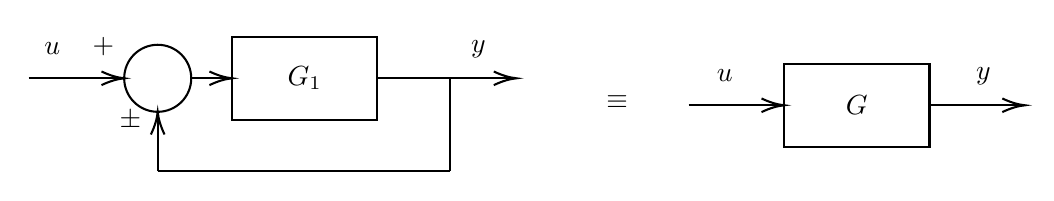
\begin{tikzpicture}[x=0.75pt,y=0.75pt,yscale=-1,xscale=1]
	%uncomment if require: \path (0,142); %set diagram left start at 0, and has height of 142
	
	%Shape: Rectangle [id:dp7400774739258154] 
	\draw   (176.5,52.5) -- (246.5,52.5) -- (246.5,92.5) -- (176.5,92.5) -- cycle ;
	%Straight Lines [id:da932624228102461] 
	\draw    (78.5,72.5) -- (122.5,72.5) ;
	\draw [shift={(124.5,72.5)}, rotate = 180] [color={rgb, 255:red, 0; green, 0; blue, 0 }  ][line width=0.75]    (10.93,-3.29) .. controls (6.95,-1.4) and (3.31,-0.3) .. (0,0) .. controls (3.31,0.3) and (6.95,1.4) .. (10.93,3.29)   ;
	
	%Straight Lines [id:da4699870099733312] 
	\draw    (246.8,72.5) -- (311.5,72.5) ;
	\draw [shift={(313.5,72.5)}, rotate = 180] [color={rgb, 255:red, 0; green, 0; blue, 0 }  ][line width=0.75]    (10.93,-3.29) .. controls (6.95,-1.4) and (3.31,-0.3) .. (0,0) .. controls (3.31,0.3) and (6.95,1.4) .. (10.93,3.29)   ;
	
	%Straight Lines [id:da5969384975066614] 
	\draw    (156.8,72.5) -- (174.5,72.5) ;
	\draw [shift={(176.5,72.5)}, rotate = 180] [color={rgb, 255:red, 0; green, 0; blue, 0 }  ][line width=0.75]    (10.93,-3.29) .. controls (6.95,-1.4) and (3.31,-0.3) .. (0,0) .. controls (3.31,0.3) and (6.95,1.4) .. (10.93,3.29)   ;
	
	%Shape: Rectangle [id:dp3907855174239989] 
	\draw   (442.5,65.5) -- (512.5,65.5) -- (512.5,105.5) -- (442.5,105.5) -- cycle ;
	%Straight Lines [id:da24051365316018458] 
	\draw    (512.5,85.5) -- (556.5,85.5) ;
	\draw [shift={(558.5,85.5)}, rotate = 180] [color={rgb, 255:red, 0; green, 0; blue, 0 }  ][line width=0.75]    (10.93,-3.29) .. controls (6.95,-1.4) and (3.31,-0.3) .. (0,0) .. controls (3.31,0.3) and (6.95,1.4) .. (10.93,3.29)   ;
	
	%Straight Lines [id:da7089642197357304] 
	\draw    (396.5,85.5) -- (440.5,85.5) ;
	\draw [shift={(442.5,85.5)}, rotate = 180] [color={rgb, 255:red, 0; green, 0; blue, 0 }  ][line width=0.75]    (10.93,-3.29) .. controls (6.95,-1.4) and (3.31,-0.3) .. (0,0) .. controls (3.31,0.3) and (6.95,1.4) .. (10.93,3.29)   ;
	
	%Flowchart: Connector [id:dp8994365253854315] 
	\draw   (124.5,72.5) .. controls (124.5,63.58) and (131.73,56.35) .. (140.65,56.35) .. controls (149.57,56.35) and (156.8,63.58) .. (156.8,72.5) .. controls (156.8,81.42) and (149.57,88.65) .. (140.65,88.65) .. controls (131.73,88.65) and (124.5,81.42) .. (124.5,72.5) -- cycle ;
	%Straight Lines [id:da4632748540731406] 
	\draw    (140.65,117.33) -- (140.65,90.65) ;
	\draw [shift={(140.65,88.65)}, rotate = 450] [color={rgb, 255:red, 0; green, 0; blue, 0 }  ][line width=0.75]    (10.93,-3.29) .. controls (6.95,-1.4) and (3.31,-0.3) .. (0,0) .. controls (3.31,0.3) and (6.95,1.4) .. (10.93,3.29)   ;
	
	%Straight Lines [id:da9141929721528332] 
	\draw    (140.65,117.33) -- (281.5,117.33) ;
	
	
	%Straight Lines [id:da19831991360071943] 
	\draw    (281.5,117.33) -- (281.5,72.5) ;
	
	
	
	% Text Node
	\draw (211.5,72.5) node   {$G_{1}$};
	% Text Node
	\draw (477.5,85.5) node   {$G$};
	% Text Node
	\draw (114.5,57) node   {$+$};
	% Text Node
	\draw (127.5,93) node   {$\pm $};
	% Text Node
	\draw (362,84) node   {$\equiv $};
	% Text Node
	\draw (413.84,71.33) node   {$u$};
	% Text Node
	\draw (538.52,71.33) node   {$y$};
	% Text Node
	\draw (89.82,58.33) node   {$u$};
	% Text Node
	\draw (295.18,58.33) node   {$y$};
	
	
	\end{tikzpicture}
\end{center}
\[
G = \frac{G_1}{1\mp G_1}
\]

\subsection{Spostamento punto di prelievo}
\begin{center}
	
	
	\tikzset{every picture/.style={line width=0.75pt}} %set default line width to 0.75pt        
	
	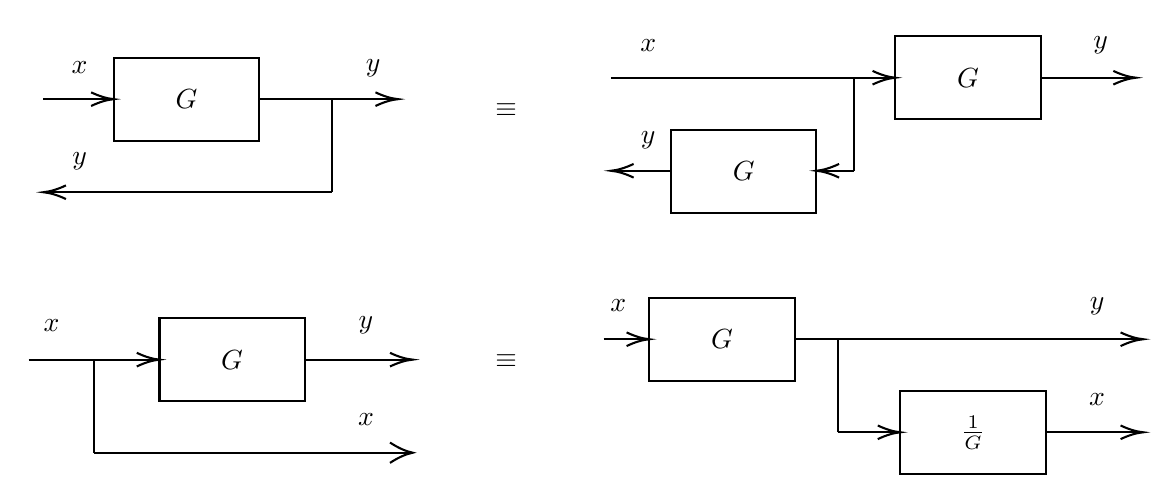
\begin{tikzpicture}[x=0.75pt,y=0.75pt,yscale=-1,xscale=1]
	%uncomment if require: \path (0,373.34375); %set diagram left start at 0, and has height of 373.34375
	
	%Shape: Rectangle [id:dp310777363660222] 
	\draw   (133.5,70.83) -- (203.5,70.83) -- (203.5,110.83) -- (133.5,110.83) -- cycle ;
	%Straight Lines [id:da518533906470976] 
	\draw    (203.8,90.83) -- (268.5,90.83) ;
	\draw [shift={(270.5,90.83)}, rotate = 180] [color={rgb, 255:red, 0; green, 0; blue, 0 }  ][line width=0.75]    (10.93,-3.29) .. controls (6.95,-1.4) and (3.31,-0.3) .. (0,0) .. controls (3.31,0.3) and (6.95,1.4) .. (10.93,3.29)   ;
	
	%Straight Lines [id:da9728704924925071] 
	\draw    (99.5,90.83) -- (131.5,90.83) ;
	\draw [shift={(133.5,90.83)}, rotate = 180] [color={rgb, 255:red, 0; green, 0; blue, 0 }  ][line width=0.75]    (10.93,-3.29) .. controls (6.95,-1.4) and (3.31,-0.3) .. (0,0) .. controls (3.31,0.3) and (6.95,1.4) .. (10.93,3.29)   ;
	
	%Straight Lines [id:da849728541549386] 
	\draw    (101.5,135.67) -- (238.5,135.67) ;
	
	\draw [shift={(99.5,135.67)}, rotate = 0] [color={rgb, 255:red, 0; green, 0; blue, 0 }  ][line width=0.75]    (10.93,-3.29) .. controls (6.95,-1.4) and (3.31,-0.3) .. (0,0) .. controls (3.31,0.3) and (6.95,1.4) .. (10.93,3.29)   ;
	%Straight Lines [id:da849509594002716] 
	\draw    (238.5,135.67) -- (238.5,90.83) ;
	
	
	%Shape: Rectangle [id:dp0636525664044818] 
	\draw   (510,60.5) -- (580,60.5) -- (580,100.5) -- (510,100.5) -- cycle ;
	%Straight Lines [id:da9359886342204105] 
	\draw    (580,80.5) -- (624,80.5) ;
	\draw [shift={(626,80.5)}, rotate = 180] [color={rgb, 255:red, 0; green, 0; blue, 0 }  ][line width=0.75]    (10.93,-3.29) .. controls (6.95,-1.4) and (3.31,-0.3) .. (0,0) .. controls (3.31,0.3) and (6.95,1.4) .. (10.93,3.29)   ;
	
	%Straight Lines [id:da7528345880250529] 
	\draw    (373,80.5) -- (508,80.5) ;
	\draw [shift={(510,80.5)}, rotate = 180] [color={rgb, 255:red, 0; green, 0; blue, 0 }  ][line width=0.75]    (10.93,-3.29) .. controls (6.95,-1.4) and (3.31,-0.3) .. (0,0) .. controls (3.31,0.3) and (6.95,1.4) .. (10.93,3.29)   ;
	
	%Straight Lines [id:da17571556748329886] 
	\draw    (474,125.33) -- (490,125.33) ;
	
	\draw [shift={(472,125.33)}, rotate = 0] [color={rgb, 255:red, 0; green, 0; blue, 0 }  ][line width=0.75]    (10.93,-3.29) .. controls (6.95,-1.4) and (3.31,-0.3) .. (0,0) .. controls (3.31,0.3) and (6.95,1.4) .. (10.93,3.29)   ;
	%Straight Lines [id:da08197563882695591] 
	\draw    (490,125.33) -- (490,80.5) ;
	
	
	%Shape: Rectangle [id:dp012916245589069453] 
	\draw   (402,105.5) -- (472,105.5) -- (472,145.5) -- (402,145.5) -- cycle ;
	%Straight Lines [id:da6813463346049113] 
	\draw    (375,125.33) -- (402,125.33) ;
	
	\draw [shift={(373,125.33)}, rotate = 0] [color={rgb, 255:red, 0; green, 0; blue, 0 }  ][line width=0.75]    (10.93,-3.29) .. controls (6.95,-1.4) and (3.31,-0.3) .. (0,0) .. controls (3.31,0.3) and (6.95,1.4) .. (10.93,3.29)   ;
	%Shape: Rectangle [id:dp4045732441435752] 
	\draw   (155.5,196.33) -- (225.5,196.33) -- (225.5,236.33) -- (155.5,236.33) -- cycle ;
	
	%Straight Lines [id:da016496853100529174] 
	\draw    (225.5,216.33) -- (275.5,216.33) ;
	\draw [shift={(277.5,216.33)}, rotate = 180] [color={rgb, 255:red, 0; green, 0; blue, 0 }  ][line width=0.75]    (10.93,-3.29) .. controls (6.95,-1.4) and (3.31,-0.3) .. (0,0) .. controls (3.31,0.3) and (6.95,1.4) .. (10.93,3.29)   ;
	
	%Straight Lines [id:da7057615327790325] 
	\draw    (92.5,216.33) -- (153.5,216.33) ;
	\draw [shift={(155.5,216.33)}, rotate = 180] [color={rgb, 255:red, 0; green, 0; blue, 0 }  ][line width=0.75]    (10.93,-3.29) .. controls (6.95,-1.4) and (3.31,-0.3) .. (0,0) .. controls (3.31,0.3) and (6.95,1.4) .. (10.93,3.29)   ;
	
	%Straight Lines [id:da6322832188032141] 
	\draw    (124,261.17) -- (275.5,261.17) ;
	\draw [shift={(277.5,261.17)}, rotate = 180] [color={rgb, 255:red, 0; green, 0; blue, 0 }  ][line width=0.75]    (10.93,-4.9) .. controls (6.95,-2.3) and (3.31,-0.67) .. (0,0) .. controls (3.31,0.67) and (6.95,2.3) .. (10.93,4.9)   ;
	
	%Straight Lines [id:da5609261518862365] 
	\draw    (124,261.17) -- (124,216.33) ;
	
	
	%Shape: Rectangle [id:dp3821800884740554] 
	\draw   (391.5,186.5) -- (461.5,186.5) -- (461.5,226.5) -- (391.5,226.5) -- cycle ;
	
	%Straight Lines [id:da1809455253187493] 
	\draw    (461.5,206.5) -- (627.5,206.5) ;
	\draw [shift={(629.5,206.5)}, rotate = 180] [color={rgb, 255:red, 0; green, 0; blue, 0 }  ][line width=0.75]    (10.93,-3.29) .. controls (6.95,-1.4) and (3.31,-0.3) .. (0,0) .. controls (3.31,0.3) and (6.95,1.4) .. (10.93,3.29)   ;
	
	%Straight Lines [id:da7659461130654208] 
	\draw    (510.5,251.33) -- (482.5,251.33) ;
	
	\draw [shift={(512.5,251.33)}, rotate = 180] [color={rgb, 255:red, 0; green, 0; blue, 0 }  ][line width=0.75]    (10.93,-3.29) .. controls (6.95,-1.4) and (3.31,-0.3) .. (0,0) .. controls (3.31,0.3) and (6.95,1.4) .. (10.93,3.29)   ;
	%Straight Lines [id:da9860283239601588] 
	\draw    (482.5,251.33) -- (482.5,206.5) ;
	
	
	%Shape: Rectangle [id:dp04900183758979271] 
	\draw   (512.5,231.5) -- (582.5,231.5) -- (582.5,271.5) -- (512.5,271.5) -- cycle ;
	%Straight Lines [id:da7589011428064532] 
	\draw    (627.5,251.33) -- (582.5,251.33) ;
	
	\draw [shift={(629.5,251.33)}, rotate = 180] [color={rgb, 255:red, 0; green, 0; blue, 0 }  ][line width=0.75]    (10.93,-3.29) .. controls (6.95,-1.4) and (3.31,-0.3) .. (0,0) .. controls (3.31,0.3) and (6.95,1.4) .. (10.93,3.29)   ;
	%Straight Lines [id:da3280510664161822] 
	\draw    (369.5,206.5) -- (389.5,206.5) ;
	\draw [shift={(391.5,206.5)}, rotate = 180] [color={rgb, 255:red, 0; green, 0; blue, 0 }  ][line width=0.75]    (10.93,-3.29) .. controls (6.95,-1.4) and (3.31,-0.3) .. (0,0) .. controls (3.31,0.3) and (6.95,1.4) .. (10.93,3.29)   ;
	
	
	% Text Node
	\draw (168.5,90.83) node   {$G$};
	% Text Node
	\draw (117,75.83) node   {$x$};
	% Text Node
	\draw (117,120.83) node   {$y$};
	% Text Node
	\draw (258.5,75.83) node   {$y$};
	% Text Node
	\draw (322.5,96.25) node   {$\equiv $};
	% Text Node
	\draw (545,80.5) node   {$G$};
	% Text Node
	\draw (391,65) node   {$x$};
	% Text Node
	\draw (391,110.5) node   {$y$};
	% Text Node
	\draw (609,65) node   {$y$};
	% Text Node
	\draw (437,125.5) node   {$G$};
	% Text Node
	\draw (190.5,216.33) node   {$G$};
	% Text Node
	\draw (103.5,199.83) node   {$x$};
	% Text Node
	\draw (255,245.33) node   {$x$};
	% Text Node
	\draw (255,199.83) node   {$y$};
	% Text Node
	\draw (426.5,206.5) node   {$G$};
	% Text Node
	\draw (376.5,190.5) node   {$x$};
	% Text Node
	\draw (607.25,190.5) node   {$y$};
	% Text Node
	\draw (547.5,251.5) node   {$\frac{1}{G}$};
	% Text Node
	\draw (322.5,217.25) node   {$\equiv $};
	% Text Node
	\draw (607.25,235.58) node   {$x$};
	
	
	\end{tikzpicture}
\end{center}

\subsection{Spostamento nodi}
\begin{center}
	
	
	\tikzset{every picture/.style={line width=0.75pt}} %set default line width to 0.75pt        
	
	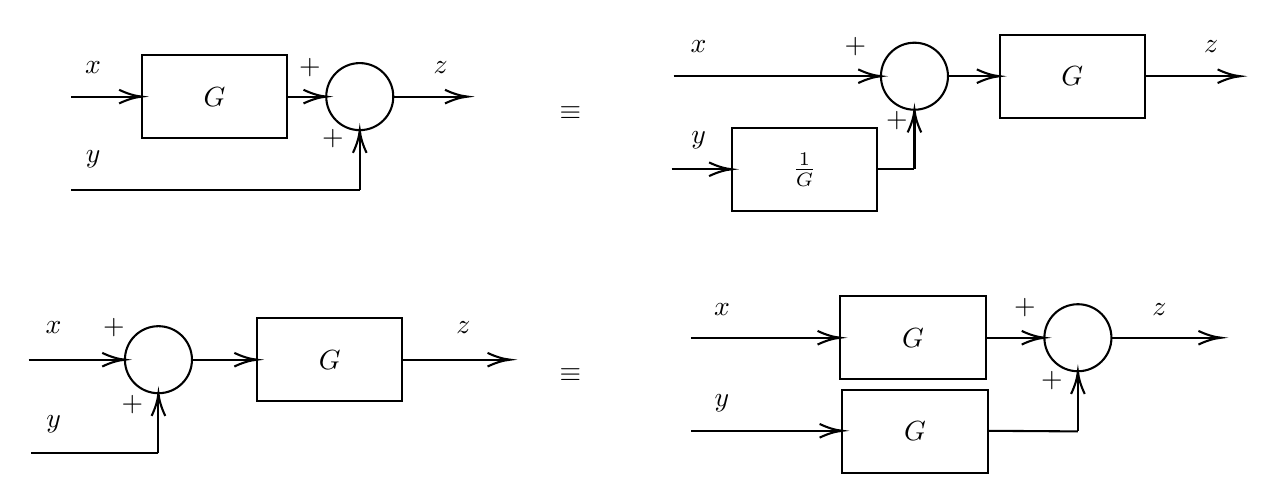
\begin{tikzpicture}[x=0.75pt,y=0.75pt,yscale=-1,xscale=1]
	%uncomment if require: \path (0,457); %set diagram left start at 0, and has height of 457
	
	%Shape: Rectangle [id:dp6135595090947077] 
	\draw   (79,92.33) -- (149,92.33) -- (149,132.33) -- (79,132.33) -- cycle ;
	%Straight Lines [id:da3626055804507693] 
	\draw    (200.15,112.33) -- (234,112.33) ;
	\draw [shift={(236,112.33)}, rotate = 180] [color={rgb, 255:red, 0; green, 0; blue, 0 }  ][line width=0.75]    (10.93,-3.29) .. controls (6.95,-1.4) and (3.31,-0.3) .. (0,0) .. controls (3.31,0.3) and (6.95,1.4) .. (10.93,3.29)   ;
	
	%Straight Lines [id:da41744824271159975] 
	\draw    (45,112.33) -- (77,112.33) ;
	\draw [shift={(79,112.33)}, rotate = 180] [color={rgb, 255:red, 0; green, 0; blue, 0 }  ][line width=0.75]    (10.93,-3.29) .. controls (6.95,-1.4) and (3.31,-0.3) .. (0,0) .. controls (3.31,0.3) and (6.95,1.4) .. (10.93,3.29)   ;
	
	%Straight Lines [id:da578409866482468] 
	\draw    (45,157.17) -- (184,157.17) ;
	
	
	%Straight Lines [id:da5740906504082484] 
	\draw    (184,157.17) -- (184,130.48) ;
	\draw [shift={(184,128.48)}, rotate = 450] [color={rgb, 255:red, 0; green, 0; blue, 0 }  ][line width=0.75]    (10.93,-3.29) .. controls (6.95,-1.4) and (3.31,-0.3) .. (0,0) .. controls (3.31,0.3) and (6.95,1.4) .. (10.93,3.29)   ;
	
	%Flowchart: Connector [id:dp20292908152923217] 
	\draw   (167.85,112.33) .. controls (167.85,103.41) and (175.08,96.18) .. (184,96.18) .. controls (192.92,96.18) and (200.15,103.41) .. (200.15,112.33) .. controls (200.15,121.25) and (192.92,128.48) .. (184,128.48) .. controls (175.08,128.48) and (167.85,121.25) .. (167.85,112.33) -- cycle ;
	%Straight Lines [id:da8700255313528944] 
	\draw    (149.3,112.33) -- (165.85,112.33) ;
	\draw [shift={(167.85,112.33)}, rotate = 180] [color={rgb, 255:red, 0; green, 0; blue, 0 }  ][line width=0.75]    (10.93,-3.29) .. controls (6.95,-1.4) and (3.31,-0.3) .. (0,0) .. controls (3.31,0.3) and (6.95,1.4) .. (10.93,3.29)   ;
	
	
	%Shape: Rectangle [id:dp009097652213897467] 
	\draw   (492.25,82.5) -- (562.25,82.5) -- (562.25,122.5) -- (492.25,122.5) -- cycle ;
	%Straight Lines [id:da8515328769624075] 
	\draw    (562.25,102.5) -- (606.25,102.5) ;
	\draw [shift={(608.25,102.5)}, rotate = 180] [color={rgb, 255:red, 0; green, 0; blue, 0 }  ][line width=0.75]    (10.93,-3.29) .. controls (6.95,-1.4) and (3.31,-0.3) .. (0,0) .. controls (3.31,0.3) and (6.95,1.4) .. (10.93,3.29)   ;
	
	%Straight Lines [id:da9961697033989048] 
	\draw    (467.4,102.5) -- (490.25,102.5) ;
	\draw [shift={(492.25,102.5)}, rotate = 180] [color={rgb, 255:red, 0; green, 0; blue, 0 }  ][line width=0.75]    (10.93,-3.29) .. controls (6.95,-1.4) and (3.31,-0.3) .. (0,0) .. controls (3.31,0.3) and (6.95,1.4) .. (10.93,3.29)   ;
	
	%Straight Lines [id:da669982976045326] 
	\draw    (433.25,147.33) -- (451.25,147.33) ;
	
	
	%Straight Lines [id:da508943180922476] 
	\draw    (451.25,147.33) -- (451.25,120.65) ;
	\draw [shift={(451.25,118.65)}, rotate = 450] [color={rgb, 255:red, 0; green, 0; blue, 0 }  ][line width=0.75]    (10.93,-3.29) .. controls (6.95,-1.4) and (3.31,-0.3) .. (0,0) .. controls (3.31,0.3) and (6.95,1.4) .. (10.93,3.29)   ;
	
	%Shape: Rectangle [id:dp34034711072843415] 
	\draw   (363.25,127.5) -- (433.25,127.5) -- (433.25,167.5) -- (363.25,167.5) -- cycle ;
	%Straight Lines [id:da9645474122482631] 
	\draw    (334.25,147.33) -- (361.25,147.33) ;
	\draw [shift={(363.25,147.33)}, rotate = 180] [color={rgb, 255:red, 0; green, 0; blue, 0 }  ][line width=0.75]    (10.93,-3.29) .. controls (6.95,-1.4) and (3.31,-0.3) .. (0,0) .. controls (3.31,0.3) and (6.95,1.4) .. (10.93,3.29)   ;
	
	%Flowchart: Connector [id:dp6193436001401342] 
	\draw   (435.1,102.5) .. controls (435.1,93.58) and (442.33,86.35) .. (451.25,86.35) .. controls (460.17,86.35) and (467.4,93.58) .. (467.4,102.5) .. controls (467.4,111.42) and (460.17,118.65) .. (451.25,118.65) .. controls (442.33,118.65) and (435.1,111.42) .. (435.1,102.5) -- cycle ;
	%Straight Lines [id:da6473663361423925] 
	\draw    (335.25,102.5) -- (433.1,102.5) ;
	\draw [shift={(435.1,102.5)}, rotate = 180] [color={rgb, 255:red, 0; green, 0; blue, 0 }  ][line width=0.75]    (10.93,-3.29) .. controls (6.95,-1.4) and (3.31,-0.3) .. (0,0) .. controls (3.31,0.3) and (6.95,1.4) .. (10.93,3.29)   ;
	
	
	%Shape: Rectangle [id:dp712303047260725] 
	\draw   (134.5,219.08) -- (204.5,219.08) -- (204.5,259.08) -- (134.5,259.08) -- cycle ;
	
	%Straight Lines [id:da9828635155497281] 
	\draw    (204.5,239.08) -- (254.5,239.08) ;
	\draw [shift={(256.5,239.08)}, rotate = 180] [color={rgb, 255:red, 0; green, 0; blue, 0 }  ][line width=0.75]    (10.93,-3.29) .. controls (6.95,-1.4) and (3.31,-0.3) .. (0,0) .. controls (3.31,0.3) and (6.95,1.4) .. (10.93,3.29)   ;
	
	%Straight Lines [id:da21237269037472162] 
	\draw    (103.15,239.08) -- (132.5,239.08) ;
	\draw [shift={(134.5,239.08)}, rotate = 180] [color={rgb, 255:red, 0; green, 0; blue, 0 }  ][line width=0.75]    (10.93,-3.29) .. controls (6.95,-1.4) and (3.31,-0.3) .. (0,0) .. controls (3.31,0.3) and (6.95,1.4) .. (10.93,3.29)   ;
	
	%Straight Lines [id:da011840201342099288] 
	\draw    (87,283.92) -- (25.5,283.92) ;
	
	
	%Straight Lines [id:da22460806935495237] 
	\draw    (87,283.92) -- (87,257.23) ;
	\draw [shift={(87,255.23)}, rotate = 450] [color={rgb, 255:red, 0; green, 0; blue, 0 }  ][line width=0.75]    (10.93,-3.29) .. controls (6.95,-1.4) and (3.31,-0.3) .. (0,0) .. controls (3.31,0.3) and (6.95,1.4) .. (10.93,3.29)   ;
	
	%Flowchart: Connector [id:dp26403356946412915] 
	\draw   (70.85,239.08) .. controls (70.85,230.16) and (78.08,222.93) .. (87,222.93) .. controls (95.92,222.93) and (103.15,230.16) .. (103.15,239.08) .. controls (103.15,248) and (95.92,255.23) .. (87,255.23) .. controls (78.08,255.23) and (70.85,248) .. (70.85,239.08) -- cycle ;
	%Straight Lines [id:da7513151428837639] 
	\draw    (24.5,239.08) -- (68.85,239.08) ;
	\draw [shift={(70.85,239.08)}, rotate = 180] [color={rgb, 255:red, 0; green, 0; blue, 0 }  ][line width=0.75]    (10.93,-3.29) .. controls (6.95,-1.4) and (3.31,-0.3) .. (0,0) .. controls (3.31,0.3) and (6.95,1.4) .. (10.93,3.29)   ;
	
	
	%Shape: Rectangle [id:dp14816381333465634] 
	\draw   (415.5,208.5) -- (485.5,208.5) -- (485.5,248.5) -- (415.5,248.5) -- cycle ;
	
	%Straight Lines [id:da24019931650280113] 
	\draw    (485.5,228.5) -- (511.85,228.5) ;
	\draw [shift={(513.85,228.5)}, rotate = 180] [color={rgb, 255:red, 0; green, 0; blue, 0 }  ][line width=0.75]    (10.93,-3.29) .. controls (6.95,-1.4) and (3.31,-0.3) .. (0,0) .. controls (3.31,0.3) and (6.95,1.4) .. (10.93,3.29)   ;
	
	%Straight Lines [id:da039464805055267504] 
	\draw    (530,273.63) -- (486.5,273.33) ;
	
	
	%Straight Lines [id:da08890940325580954] 
	\draw    (530,273.63) -- (530,246.65) ;
	\draw [shift={(530,244.65)}, rotate = 450] [color={rgb, 255:red, 0; green, 0; blue, 0 }  ][line width=0.75]    (10.93,-3.29) .. controls (6.95,-1.4) and (3.31,-0.3) .. (0,0) .. controls (3.31,0.3) and (6.95,1.4) .. (10.93,3.29)   ;
	
	%Shape: Rectangle [id:dp4150429324233136] 
	\draw   (416.5,253.5) -- (486.5,253.5) -- (486.5,293.5) -- (416.5,293.5) -- cycle ;
	%Straight Lines [id:da8006311284636038] 
	\draw    (414.5,273.33) -- (343.5,273.33) ;
	
	\draw [shift={(416.5,273.33)}, rotate = 180] [color={rgb, 255:red, 0; green, 0; blue, 0 }  ][line width=0.75]    (10.93,-3.29) .. controls (6.95,-1.4) and (3.31,-0.3) .. (0,0) .. controls (3.31,0.3) and (6.95,1.4) .. (10.93,3.29)   ;
	%Straight Lines [id:da5766908177542442] 
	\draw    (343.5,228.5) -- (413.5,228.5) ;
	\draw [shift={(415.5,228.5)}, rotate = 180] [color={rgb, 255:red, 0; green, 0; blue, 0 }  ][line width=0.75]    (10.93,-3.29) .. controls (6.95,-1.4) and (3.31,-0.3) .. (0,0) .. controls (3.31,0.3) and (6.95,1.4) .. (10.93,3.29)   ;
	
	%Flowchart: Connector [id:dp8405559687615076] 
	\draw   (513.85,228.5) .. controls (513.85,219.58) and (521.08,212.35) .. (530,212.35) .. controls (538.92,212.35) and (546.15,219.58) .. (546.15,228.5) .. controls (546.15,237.42) and (538.92,244.65) .. (530,244.65) .. controls (521.08,244.65) and (513.85,237.42) .. (513.85,228.5) -- cycle ;
	%Straight Lines [id:da9465923155315663] 
	\draw    (546.15,228.5) -- (597,228.5) ;
	\draw [shift={(599,228.5)}, rotate = 180] [color={rgb, 255:red, 0; green, 0; blue, 0 }  ][line width=0.75]    (10.93,-3.29) .. controls (6.95,-1.4) and (3.31,-0.3) .. (0,0) .. controls (3.31,0.3) and (6.95,1.4) .. (10.93,3.29)   ;
	
	
	
	% Text Node
	\draw (285.5,120.5) node   {$\equiv $};
	% Text Node
	\draw (285.5,246.5) node   {$\equiv $};
	% Text Node
	\draw (358.5,215) node   {$x$};
	% Text Node
	\draw (569.25,215) node   {$z$};
	% Text Node
	\draw (451.5,273.5) node   {$G$};
	% Text Node
	\draw (450.5,228.5) node   {$G$};
	% Text Node
	\draw (36.5,223.58) node   {$x$};
	% Text Node
	\draw (36.5,270.08) node   {$y$};
	% Text Node
	\draw (234,223.58) node   {$z$};
	% Text Node
	\draw (169.5,239.08) node   {$G$};
	% Text Node
	\draw (527.25,102.5) node   {$G$};
	% Text Node
	\draw (347.25,88) node   {$x$};
	% Text Node
	\draw (347.25,133.5) node   {$y$};
	% Text Node
	\draw (594.25,88) node   {$z$};
	% Text Node
	\draw (398.25,147.5) node   {$\frac{1}{G}$};
	% Text Node
	\draw (114,112.33) node   {$G$};
	% Text Node
	\draw (55.5,98.33) node   {$x$};
	% Text Node
	\draw (55.5,142.33) node   {$y$};
	% Text Node
	\draw (223,98.33) node   {$z$};
	% Text Node
	\draw (160,98.5) node   {$+$};
	% Text Node
	\draw (171,132.5) node   {$+$};
	% Text Node
	\draw (65.5,223.75) node   {$+$};
	% Text Node
	\draw (74.5,260.75) node   {$+$};
	% Text Node
	\draw (358.5,260) node   {$y$};
	% Text Node
	\draw (504.5,214) node   {$+$};
	% Text Node
	\draw (517.5,249) node   {$+$};
	% Text Node
	\draw (422.75,88) node   {$+$};
	% Text Node
	\draw (442.75,124) node   {$+$};
	
	
	\end{tikzpicture}
\end{center}

\section{Schemi a Flusso}

È una rappresentazione con linee orientate:

\begin{center}
	
	
	\tikzset{every picture/.style={line width=0.75pt}} %set default line width to 0.75pt        
	
	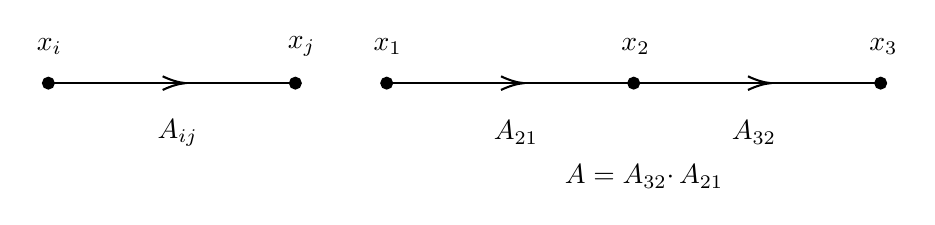
\begin{tikzpicture}[x=0.75pt,y=0.75pt,yscale=-1,xscale=1]
	%uncomment if require: \path (0,300); %set diagram left start at 0, and has height of 300
	
	%Straight Lines [id:da2645604679508091] 
	\draw    (100,127) -- (164,127) ;
	\draw [shift={(166,127)}, rotate = 180] [color={rgb, 255:red, 0; green, 0; blue, 0 }  ][line width=0.75]    (10.93,-3.29) .. controls (6.95,-1.4) and (3.31,-0.3) .. (0,0) .. controls (3.31,0.3) and (6.95,1.4) .. (10.93,3.29)   ;
	
	%Straight Lines [id:da5282887023752798] 
	\draw    (166,127) -- (219,127) ;
	
	
	%Flowchart: Connector [id:dp24093442897466288] 
	\draw  [fill={rgb, 255:red, 0; green, 0; blue, 0 }  ,fill opacity=1 ] (97.39,127) .. controls (97.39,125.56) and (98.56,124.39) .. (100,124.39) .. controls (101.44,124.39) and (102.61,125.56) .. (102.61,127) .. controls (102.61,128.44) and (101.44,129.61) .. (100,129.61) .. controls (98.56,129.61) and (97.39,128.44) .. (97.39,127) -- cycle ;
	%Flowchart: Connector [id:dp09137978863303431] 
	\draw  [fill={rgb, 255:red, 0; green, 0; blue, 0 }  ,fill opacity=1 ] (216.39,127) .. controls (216.39,125.56) and (217.56,124.39) .. (219,124.39) .. controls (220.44,124.39) and (221.61,125.56) .. (221.61,127) .. controls (221.61,128.44) and (220.44,129.61) .. (219,129.61) .. controls (217.56,129.61) and (216.39,128.44) .. (216.39,127) -- cycle ;
	%Straight Lines [id:da5682374240056367] 
	\draw    (263,127) -- (327,127) ;
	\draw [shift={(329,127)}, rotate = 180] [color={rgb, 255:red, 0; green, 0; blue, 0 }  ][line width=0.75]    (10.93,-3.29) .. controls (6.95,-1.4) and (3.31,-0.3) .. (0,0) .. controls (3.31,0.3) and (6.95,1.4) .. (10.93,3.29)   ;
	
	%Straight Lines [id:da9888198098011782] 
	\draw    (329,127) -- (382,127) ;
	
	
	%Flowchart: Connector [id:dp31773307782267945] 
	\draw  [fill={rgb, 255:red, 0; green, 0; blue, 0 }  ,fill opacity=1 ] (260.39,127) .. controls (260.39,125.56) and (261.56,124.39) .. (263,124.39) .. controls (264.44,124.39) and (265.61,125.56) .. (265.61,127) .. controls (265.61,128.44) and (264.44,129.61) .. (263,129.61) .. controls (261.56,129.61) and (260.39,128.44) .. (260.39,127) -- cycle ;
	%Flowchart: Connector [id:dp04076917753662146] 
	\draw  [fill={rgb, 255:red, 0; green, 0; blue, 0 }  ,fill opacity=1 ] (379.39,127) .. controls (379.39,125.56) and (380.56,124.39) .. (382,124.39) .. controls (383.44,124.39) and (384.61,125.56) .. (384.61,127) .. controls (384.61,128.44) and (383.44,129.61) .. (382,129.61) .. controls (380.56,129.61) and (379.39,128.44) .. (379.39,127) -- cycle ;
	%Straight Lines [id:da09323604628620097] 
	\draw    (382,127) -- (446,127) ;
	\draw [shift={(448,127)}, rotate = 180] [color={rgb, 255:red, 0; green, 0; blue, 0 }  ][line width=0.75]    (10.93,-3.29) .. controls (6.95,-1.4) and (3.31,-0.3) .. (0,0) .. controls (3.31,0.3) and (6.95,1.4) .. (10.93,3.29)   ;
	
	%Straight Lines [id:da08735784921599854] 
	\draw    (448,127) -- (501,127) ;
	
	
	%Flowchart: Connector [id:dp6288301261150899] 
	\draw  [fill={rgb, 255:red, 0; green, 0; blue, 0 }  ,fill opacity=1 ] (498.39,127) .. controls (498.39,125.56) and (499.56,124.39) .. (501,124.39) .. controls (502.44,124.39) and (503.61,125.56) .. (503.61,127) .. controls (503.61,128.44) and (502.44,129.61) .. (501,129.61) .. controls (499.56,129.61) and (498.39,128.44) .. (498.39,127) -- cycle ;
	
	% Text Node
	\draw (162.33,150.83) node   {$A_{ij}$};
	% Text Node
	\draw (100.5,109.5) node   {$x_{i}$};
	% Text Node
	\draw (222,109.5) node   {$x_{j}$};
	% Text Node
	\draw (325.33,150.83) node   {$A_{21}$};
	% Text Node
	\draw (263.5,109.5) node   {$x_{1}$};
	% Text Node
	\draw (382.92,109.5) node   {$x_{2}$};
	% Text Node
	\draw (502.33,109.5) node   {$x_{3}$};
	% Text Node
	\draw (440,150.83) node   {$A_{32}$};
	% Text Node
	\draw (387,172) node   {$A=A_{32} \cdotp A_{21}$};
	
	
	\end{tikzpicture}
\end{center}

$ x_j, x_i $ sono i nodi, $ A_ij $ è la trasmittanza %TODO è corretto il nome?
con il primo indice l'indice del nodo di arrivo e con secondo quello di partenza

\begin{definizione}
	Cammino: qualsiasi tipo di percorso che non passa più di una volta in un nodo (inizio e fine possono essere lo stesso nodo)
	
	\begin{center}
		
		
		\tikzset{every picture/.style={line width=0.75pt}} %set default line width to 0.75pt        
		
		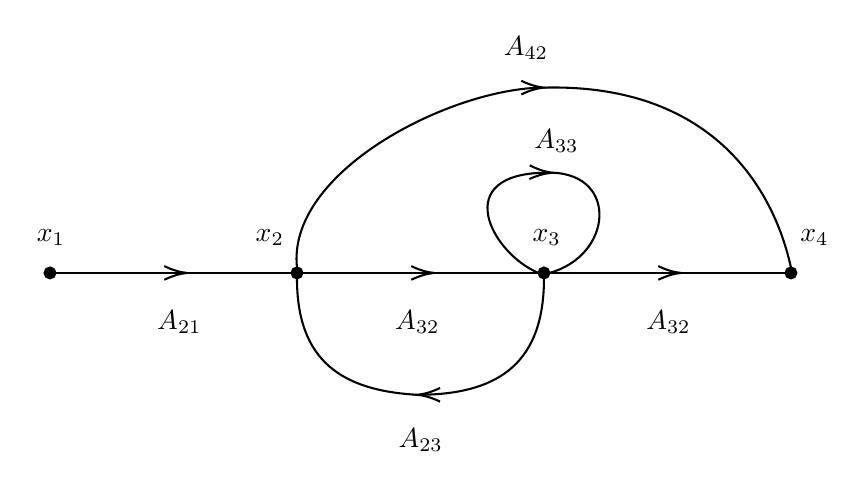
\begin{tikzpicture}[x=0.75pt,y=0.75pt,yscale=-1,xscale=1]
		%uncomment if require: \path (0,300); %set diagram left start at 0, and has height of 300
		
		%Straight Lines [id:da8105771101337726] 
		\draw    (128,137) -- (192,137) ;
		\draw [shift={(194,137)}, rotate = 180] [color={rgb, 255:red, 0; green, 0; blue, 0 }  ][line width=0.75]    (10.93,-3.29) .. controls (6.95,-1.4) and (3.31,-0.3) .. (0,0) .. controls (3.31,0.3) and (6.95,1.4) .. (10.93,3.29)   ;
		
		%Straight Lines [id:da3382037954225505] 
		\draw    (194,137) -- (247,137) ;
		
		
		%Flowchart: Connector [id:dp4469951295676833] 
		\draw  [fill={rgb, 255:red, 0; green, 0; blue, 0 }  ,fill opacity=1 ] (125.39,137) .. controls (125.39,135.56) and (126.56,134.39) .. (128,134.39) .. controls (129.44,134.39) and (130.61,135.56) .. (130.61,137) .. controls (130.61,138.44) and (129.44,139.61) .. (128,139.61) .. controls (126.56,139.61) and (125.39,138.44) .. (125.39,137) -- cycle ;
		%Flowchart: Connector [id:dp15866470914000907] 
		\draw  [fill={rgb, 255:red, 0; green, 0; blue, 0 }  ,fill opacity=1 ] (244.39,137) .. controls (244.39,135.56) and (245.56,134.39) .. (247,134.39) .. controls (248.44,134.39) and (249.61,135.56) .. (249.61,137) .. controls (249.61,138.44) and (248.44,139.61) .. (247,139.61) .. controls (245.56,139.61) and (244.39,138.44) .. (244.39,137) -- cycle ;
		%Straight Lines [id:da3380953131659412] 
		\draw    (247,137) -- (311,137) ;
		\draw [shift={(313,137)}, rotate = 180] [color={rgb, 255:red, 0; green, 0; blue, 0 }  ][line width=0.75]    (10.93,-3.29) .. controls (6.95,-1.4) and (3.31,-0.3) .. (0,0) .. controls (3.31,0.3) and (6.95,1.4) .. (10.93,3.29)   ;
		
		%Straight Lines [id:da2778079775407136] 
		\draw    (313,137) -- (366,137) ;
		
		
		%Flowchart: Connector [id:dp24437453556375677] 
		\draw  [fill={rgb, 255:red, 0; green, 0; blue, 0 }  ,fill opacity=1 ] (363.39,137) .. controls (363.39,135.56) and (364.56,134.39) .. (366,134.39) .. controls (367.44,134.39) and (368.61,135.56) .. (368.61,137) .. controls (368.61,138.44) and (367.44,139.61) .. (366,139.61) .. controls (364.56,139.61) and (363.39,138.44) .. (363.39,137) -- cycle ;
		%Straight Lines [id:da8283013982720953] 
		\draw    (366,137) -- (430,137) ;
		\draw [shift={(432,137)}, rotate = 180] [color={rgb, 255:red, 0; green, 0; blue, 0 }  ][line width=0.75]    (10.93,-3.29) .. controls (6.95,-1.4) and (3.31,-0.3) .. (0,0) .. controls (3.31,0.3) and (6.95,1.4) .. (10.93,3.29)   ;
		
		%Straight Lines [id:da24499908355444422] 
		\draw    (432,137) -- (485,137) ;
		
		
		%Flowchart: Connector [id:dp5096754872900153] 
		\draw  [fill={rgb, 255:red, 0; green, 0; blue, 0 }  ,fill opacity=1 ] (482.39,137) .. controls (482.39,135.56) and (483.56,134.39) .. (485,134.39) .. controls (486.44,134.39) and (487.61,135.56) .. (487.61,137) .. controls (487.61,138.44) and (486.44,139.61) .. (485,139.61) .. controls (483.56,139.61) and (482.39,138.44) .. (482.39,137) -- cycle ;
		%Curve Lines [id:da05030671031007761] 
		\draw    (307.38,195.7) .. controls (345.83,195.06) and (366,178.91) .. (366,139.61) ;
		
		\draw [shift={(305,195.71)}, rotate = 0] [color={rgb, 255:red, 0; green, 0; blue, 0 }  ][line width=0.75]    (10.93,-3.29) .. controls (6.95,-1.4) and (3.31,-0.3) .. (0,0) .. controls (3.31,0.3) and (6.95,1.4) .. (10.93,3.29)   ;
		%Curve Lines [id:da9411729661125996] 
		\draw    (305,195.71) .. controls (269,193.71) and (247,179.71) .. (247,139.61) ;
		
		
		%Curve Lines [id:da8637716251821868] 
		\draw    (485,134.39) .. controls (476.39,95.11) and (446,45.71) .. (366,47.71) ;
		
		
		%Curve Lines [id:da1866156970628461] 
		\draw    (368.61,137) .. controls (399,128.71) and (402,89.71) .. (370,88.71) ;
		
		
		%Curve Lines [id:da1453137619761551] 
		\draw    (364,47.74) .. controls (319.62,48.92) and (242.07,88.41) .. (247,134.39) ;
		
		\draw [shift={(366,47.71)}, rotate = 180] [color={rgb, 255:red, 0; green, 0; blue, 0 }  ][line width=0.75]    (10.93,-3.29) .. controls (6.95,-1.4) and (3.31,-0.3) .. (0,0) .. controls (3.31,0.3) and (6.95,1.4) .. (10.93,3.29)   ;
		%Curve Lines [id:da7371522355149234] 
		\draw    (367.76,88.69) .. controls (319.87,88.74) and (340.78,127.68) .. (363.39,137) ;
		
		\draw [shift={(370,88.71)}, rotate = 181.32] [color={rgb, 255:red, 0; green, 0; blue, 0 }  ][line width=0.75]    (10.93,-3.29) .. controls (6.95,-1.4) and (3.31,-0.3) .. (0,0) .. controls (3.31,0.3) and (6.95,1.4) .. (10.93,3.29)   ;
		
		% Text Node
		\draw (190.33,160.83) node   {$A_{21}$};
		% Text Node
		\draw (128.5,120) node   {$x_{1}$};
		% Text Node
		\draw (233.92,120) node   {$x_{2}$};
		% Text Node
		\draw (367.33,120) node   {$x_{3}$};
		% Text Node
		\draw (305,160.83) node   {$A_{32}$};
		% Text Node
		\draw (496.33,120) node   {$x_{4}$};
		% Text Node
		\draw (426,160.83) node   {$A_{32}$};
		% Text Node
		\draw (306.6,217.63) node   {$A_{23}$};
		% Text Node
		\draw (357.33,28.83) node   {$A_{42}$};
		% Text Node
		\draw (372,73.5) node   {$A_{33}$};
		
		
		\end{tikzpicture}
	\end{center}
	
	Esempio di cammini:
	\begin{enumerate}
		\item $ A_{21},A_{32},A_{43} $ (cammino aperto)
		\item $ A_{21},A_{42} $
		\item $ A_{32},A_{23} $ (cammino chiuso/anello)
		\item $ A_{33} $ (autoanello)
	\end{enumerate}
	
	
	
	\tikzset{every picture/.style={line width=0.75pt}} %set default line width to 0.75pt        
	
	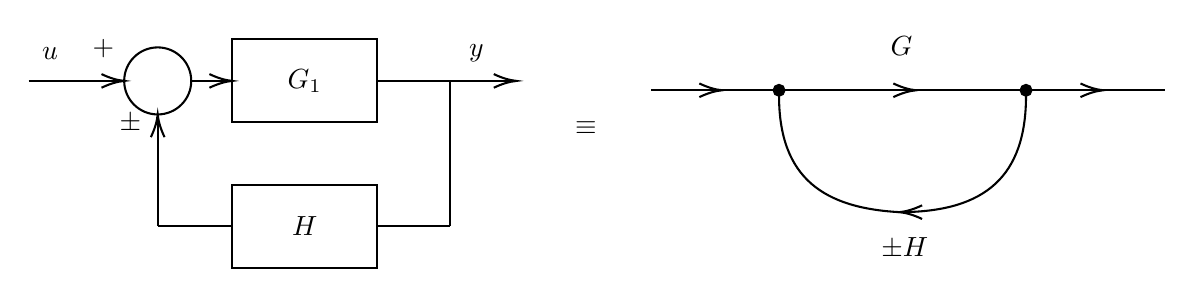
\begin{tikzpicture}[x=0.75pt,y=0.75pt,yscale=-1,xscale=1]
	%uncomment if require: \path (0,300); %set diagram left start at 0, and has height of 300
	
	%Shape: Rectangle [id:dp5584805448505255] 
	\draw   (133.5,55.07) -- (203.5,55.07) -- (203.5,95.07) -- (133.5,95.07) -- cycle ;
	%Shape: Rectangle [id:dp4639169675813819] 
	\draw   (133.5,125.07) -- (203.5,125.07) -- (203.5,165.07) -- (133.5,165.07) -- cycle ;
	%Straight Lines [id:da8973299402509956] 
	\draw    (35.5,75.07) -- (79.5,75.07) ;
	\draw [shift={(81.5,75.07)}, rotate = 180] [color={rgb, 255:red, 0; green, 0; blue, 0 }  ][line width=0.75]    (10.93,-3.29) .. controls (6.95,-1.4) and (3.31,-0.3) .. (0,0) .. controls (3.31,0.3) and (6.95,1.4) .. (10.93,3.29)   ;
	
	%Straight Lines [id:da21170135088038822] 
	\draw    (203.8,75.07) -- (268.5,75.07) ;
	\draw [shift={(270.5,75.07)}, rotate = 180] [color={rgb, 255:red, 0; green, 0; blue, 0 }  ][line width=0.75]    (10.93,-3.29) .. controls (6.95,-1.4) and (3.31,-0.3) .. (0,0) .. controls (3.31,0.3) and (6.95,1.4) .. (10.93,3.29)   ;
	
	%Straight Lines [id:da5723083322077416] 
	\draw    (113.8,75.07) -- (131.5,75.07) ;
	\draw [shift={(133.5,75.07)}, rotate = 180] [color={rgb, 255:red, 0; green, 0; blue, 0 }  ][line width=0.75]    (10.93,-3.29) .. controls (6.95,-1.4) and (3.31,-0.3) .. (0,0) .. controls (3.31,0.3) and (6.95,1.4) .. (10.93,3.29)   ;
	
	%Flowchart: Connector [id:dp7852522645677837] 
	\draw   (81.5,75.07) .. controls (81.5,66.15) and (88.73,58.92) .. (97.65,58.92) .. controls (106.57,58.92) and (113.8,66.15) .. (113.8,75.07) .. controls (113.8,83.99) and (106.57,91.22) .. (97.65,91.22) .. controls (88.73,91.22) and (81.5,83.99) .. (81.5,75.07) -- cycle ;
	%Straight Lines [id:da6466686716461845] 
	\draw    (97.65,145.07) -- (97.65,93.22) ;
	\draw [shift={(97.65,91.22)}, rotate = 450] [color={rgb, 255:red, 0; green, 0; blue, 0 }  ][line width=0.75]    (10.93,-3.29) .. controls (6.95,-1.4) and (3.31,-0.3) .. (0,0) .. controls (3.31,0.3) and (6.95,1.4) .. (10.93,3.29)   ;
	
	%Straight Lines [id:da05815677457067303] 
	\draw    (203.5,145.07) -- (238.5,145.07) ;
	
	
	%Straight Lines [id:da3233505457901875] 
	\draw    (97.65,145.07) -- (133.5,145.07) ;
	
	
	%Straight Lines [id:da01361016899977252] 
	\draw    (238.5,145.07) -- (238.5,75.07) ;
	
	
	
	%Straight Lines [id:da9489064314757574] 
	\draw    (335.35,79.58) -- (367.54,79.58) ;
	\draw [shift={(369.54,79.58)}, rotate = 180] [color={rgb, 255:red, 0; green, 0; blue, 0 }  ][line width=0.75]    (10.93,-3.29) .. controls (6.95,-1.4) and (3.31,-0.3) .. (0,0) .. controls (3.31,0.3) and (6.95,1.4) .. (10.93,3.29)   ;
	
	%Straight Lines [id:da023992851870582532] 
	\draw    (369.54,79.58) -- (397,79.58) ;
	
	
	%Flowchart: Connector [id:dp18813000644471334] 
	\draw  [fill={rgb, 255:red, 0; green, 0; blue, 0 }  ,fill opacity=1 ] (394.39,79.58) .. controls (394.39,78.14) and (395.56,76.98) .. (397,76.98) .. controls (398.44,76.98) and (399.61,78.14) .. (399.61,79.58) .. controls (399.61,81.02) and (398.44,82.19) .. (397,82.19) .. controls (395.56,82.19) and (394.39,81.02) .. (394.39,79.58) -- cycle ;
	%Straight Lines [id:da04318951705463547] 
	\draw    (397,79.58) -- (461,79.58) ;
	\draw [shift={(463,79.58)}, rotate = 180] [color={rgb, 255:red, 0; green, 0; blue, 0 }  ][line width=0.75]    (10.93,-3.29) .. controls (6.95,-1.4) and (3.31,-0.3) .. (0,0) .. controls (3.31,0.3) and (6.95,1.4) .. (10.93,3.29)   ;
	
	%Straight Lines [id:da1911166961256583] 
	\draw    (463,79.58) -- (516,79.58) ;
	
	
	%Flowchart: Connector [id:dp14709331014549343] 
	\draw  [fill={rgb, 255:red, 0; green, 0; blue, 0 }  ,fill opacity=1 ] (513.39,79.58) .. controls (513.39,78.14) and (514.56,76.98) .. (516,76.98) .. controls (517.44,76.98) and (518.61,78.14) .. (518.61,79.58) .. controls (518.61,81.02) and (517.44,82.19) .. (516,82.19) .. controls (514.56,82.19) and (513.39,81.02) .. (513.39,79.58) -- cycle ;
	%Straight Lines [id:da9901825078822903] 
	\draw    (516,79.58) -- (551.18,79.58) ;
	\draw [shift={(553.18,79.58)}, rotate = 180] [color={rgb, 255:red, 0; green, 0; blue, 0 }  ][line width=0.75]    (10.93,-3.29) .. controls (6.95,-1.4) and (3.31,-0.3) .. (0,0) .. controls (3.31,0.3) and (6.95,1.4) .. (10.93,3.29)   ;
	
	%Straight Lines [id:da9417777255935527] 
	\draw    (553.18,79.58) -- (583.03,79.58) ;
	
	
	%Curve Lines [id:da8849773075030309] 
	\draw    (457.38,138.28) .. controls (495.83,137.65) and (516,121.5) .. (516,82.19) ;
	
	\draw [shift={(455,138.3)}, rotate = 0] [color={rgb, 255:red, 0; green, 0; blue, 0 }  ][line width=0.75]    (10.93,-3.29) .. controls (6.95,-1.4) and (3.31,-0.3) .. (0,0) .. controls (3.31,0.3) and (6.95,1.4) .. (10.93,3.29)   ;
	%Curve Lines [id:da11116878216013837] 
	\draw    (455,138.3) .. controls (419,136.3) and (397,122.3) .. (397,82.19) ;
	
	
	
	
	% Text Node
	\draw (168.5,75.07) node   {$G_{1}$};
	% Text Node
	\draw (168.5,145.07) node   {$H$};
	% Text Node
	\draw (71.5,59.57) node   {$+$};
	% Text Node
	\draw (84.5,95.57) node   {$\pm $};
	% Text Node
	\draw (45.82,61.9) node   {$u$};
	% Text Node
	\draw (251.18,61.9) node   {$y$};
	% Text Node
	\draw (456,58.42) node   {$G$};
	% Text Node
	\draw (457.6,155.72) node   {$\pm H$};
	% Text Node
	\draw (304,98) node   {$\equiv $};
	
	
	\end{tikzpicture}
	
\end{definizione}
	
	

